\chapter{Preliminaries}
\label{ch:Foundations}

\section{Confidential Computing}
\label{sec:Foundations:ConfComputing}
Confidential Computing means the protection of data during computation by performing those computations in attested Trusted Execution Environments (TEE). Similarly to Trusted Computing, Confidential Computing is predominantly a marketing term and has no single definition. The following tries to establish the definition as it will be used in this thesis. Unlike Trusted Computing, which aims to establish integrity of hardware and software, Confidential Computing also aims to guarantee the authenticity. Using TEEs in the lowest layer of hardware reduces the number of trusted parties. In this case, a party could be a hardware or software vendor. Security in one abstraction layer of the compute stack is only as strong as the layers below it if no other measures are used to prevent access. Homomorphic encryption gives some additional security guarantees even if the underlying layers are not trusted. Figure \ref{fig:computestack} shows a basic compute stack with the most common layers. A bug in the hypervisor, if present, can affect the execution of the operating system and, in the worst case allow unauthorized entities to read or change the data in use.
\begin{figure}
\centering
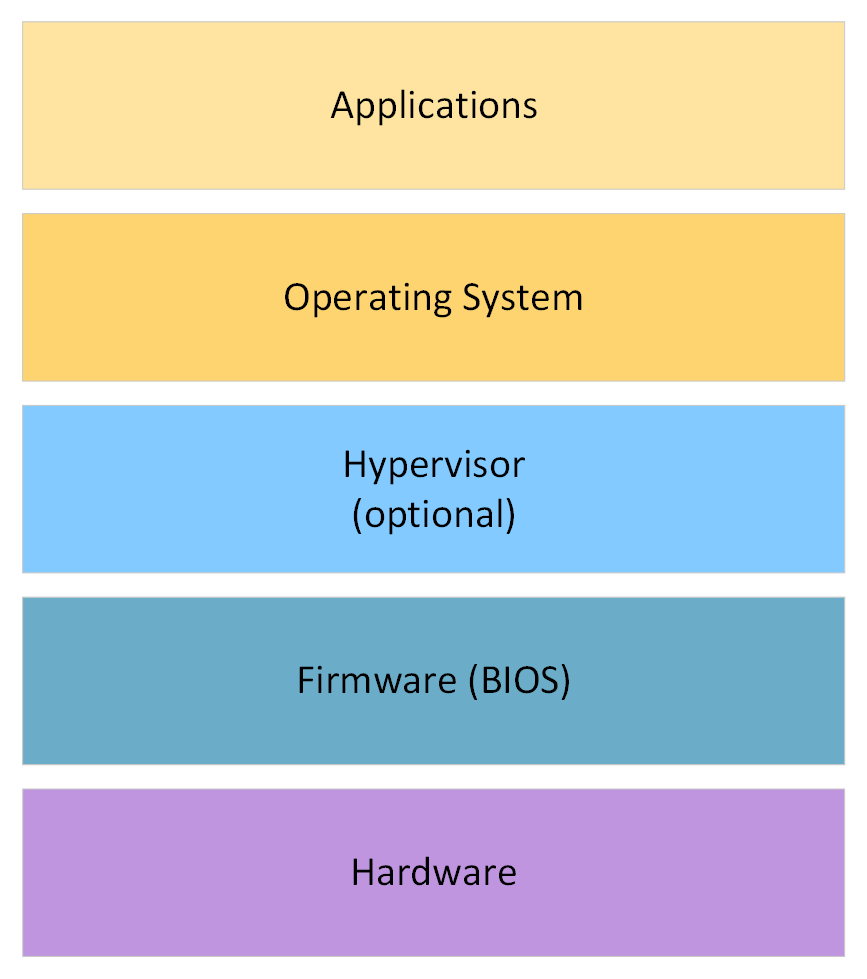
\includegraphics[width=0.5\textwidth]{figures/ComputeStack.png}
\caption{A rudimentary Compute Stack. Most layers can be split up further if needed to}
\label{fig:computestack}
\end{figure}Security in higher layers can be bypassed from lower layers. Security solutions at the hardware level can remove the operating system, device drivers, and more from the list of trusted parties. A TEE is, as defined by the Confidential Computing Consortium, an environment that provides assurance in three different properties:
\begin{itemize} 
    \item \guillemotright Data confidentiality: Unauthorized entities cannot view data while it is in use within the TEE
    \item Data integrity: Unauthorized entities cannot alter the data while it is in use within the TEE.
    \item Code integrity: Unauthorized entities cannot alter the code executing in the TEE.\guillemotleft \cite{noauthor_ccc_outreach_whitepaper_updated_november_2022pdf_2023}
\end{itemize} 
In the context of Confidential Computing, unauthorized entities include, but are not limited to, other applications on the host, the host operating system itself, as well as the hypervisor, the infrastructure owner, and anyone else with physical hardware access. 
Combined, these three attributes provide an assurance that the data are kept confidential and the calculations that are performed are correct.
Depending on the specific TEE used, there might be additional security properties, but the TEEs covered in this thesis do not have more\cite{noauthor_ccc_outreach_whitepaper_updated_november_2022pdf_2023}.

\myparagraph{Integrity Measurement Architecture}

\label{IMA}

Integrity Measurement Architecture (IMA) is a feature of the Linux kernel that ensures system integrity while the system is running. It computes the hashes of files and programs prior to their execution, provides reporting capabilities, and verifies that they adhere to a predefined list.\cite{Luo_container_ima}. IMA is recommended by the Trusted Computing Group for identity verification \cite{trusted_computing_group_tcg_2023}. According to the IMA wiki \url{https://sourceforge.net/p/linux-ima/wiki/Home/} it contains two subsystems: Measurement and Appraisal. Measurement is responsible for gathering, storing, and verifying measurements. Appraisal conducts the evaluation and auditing tasks by comparing a collected hash with a stored hash and prevents access if they do not match. IMA depends on Trusted Platform Module (TPM)\cite{Luo_container_ima}. It needs a custom initramfs or similar early boot process script capabilities to be used.

\section{Trusted Domain Extension}
One implementation of TEEs by Intel is called Trusted Domain Extensions (TDX). This section gives an overview of its building blocks, its system architecture, memory protection mechanisms, I/O model, attestation, and future features.
\subsection{TDX Building Blocks}
\label{sec:tdxBuildingBlocks}
TDX combines and extends several existing Intel technologies, including Virtualization Technology (VT), Total Memory Encryption (TME), and Software Guard Extensions (SGX). This section will give an overview the technologies and how they are used. The building blocks were also outlined in \cite{cheng_intel_2023}, to which this will give some more context.
\subsubsection{Software Guard Extension}
SGX is a set of instruction codes, which were Intels first trusted execution environment. It was intended to protect against memory bus snooping and cold boot attacks. It is still in use today to protect code and data within a so called enclave, which is a secure container, containing sensitive code and data. It can contain entire applications or even an operating system but was intended to house just small parts of an application. It is encrypted using Memory Protection Extensions a predecessor to Total Memory Encryption, which is explained in \cref{Memory Encrpytion}. Data is only decrypted inside the processor\cite{intel_corporation_overview--intel-sgx-enclave_nodate}. SGX aims to protect the confidentiality of the computation inside an enclave. SGX uses hardware-based memory encryption to ensure that the RAM of an enclave can only be accessed by authorized code. Any unauthorized attempt to access the memory will result in an exception. SGX offers both local and, more importantly, remote attestation to verify the integrity of enclaves. Local attestation establishes trust between two local enclaves, and remote attestation verifies trustworthiness to a third party entity. More on attestation can be found in \cref{TDX attestation}. On the same platform, TDX and SGX are within the same Trusted Computing Base (TCB).  Therefore, they can attest each other locally\cite{intel_corporation_dcap_2024-1}, which will become important for TDX in \cref{Pre-Attestation setup}. During its lifetime Intel SGX has had many security issues, with most of them being preventable by the application developer themself. Van Schaik et Al. provide an overview of known issues at the time of writing and ways to mitigate them \cite{sgxfail}. The same source also contains an overview of attacks that can only be prevented with microcode updates by Intel itself. SGX does not want to protect against hardware-based attacks in general but mitigates some basic ones \cite{costan_intel_2016}. What is considered a basic hardware attack will be discussed further in \cref{Threat_Model}. It wants to protect against unpriviliged and privileged software attacks as well as startup code attacks \cite{schutz_general_nodate}.
\subsubsection{Intel Virtualization Technology}
Intel VT is a set of hardware-assisted virtualization features in Intel processors that can provide improved performance, isolation, and security compared to software-based virtualization. Intel VTs features include virtualization of the CPU, memory and I/O.
Intel processors contain, depending on the architecture, either VT-x or VT-i instructions. The latter being only used on the discontinued Itanium architecture. Processors with VT-x feature an extra instruction set known as Virtual Machine Extensions (VMX), allowing virtualization control. Virtualization allows the usage of multiple isolated Virtual Machines on the same hardware. It can also allow multiple different operating systems to run in these VMs\cite{intel_corporation_intel_nodate}. VMX has two different execution modes: VMX root mode, used by the hypervisor, and VMX nonroot mode, used by the guest VMs. VMX uses a second-level address translation called Extended Page Table (EPT), which aims to eliminate the overhead from software-managed page tables \cite{uhlig_intel_2005}. The TDX Module (TDXM) runs in the new Secure Arbitration Mode (SEAM) VMX root and the TDs run in the nonroot mode. The biggest change from normal VMX to SEAM VMX is the usage of an additional Extended Page Table. With VMX the hypervisor holds only one table per guest kernel, the TDXM has two per guest TD. A protected one for private memory and another unprotected one for shared memory.
With TDX being a virtual machine-based TEE, it depends on VT to ensure isolation between its Trusted Domains (TDs)\cite{cheng_intel_2023}.
\subsubsection{Intel Total Memory Encryption}
\label{Memory Encrpytion}
Intel Total Memory Encryption (TME) is a security measure designed to protect against attackers who have physical access to the memory of a computer or direct access via a host system and attempt to steal data. TME aims to protect against some, for example bus memory probing, but not all physical attacks. Direct Memory Access attacks for example are not included.TME encrypts the entire computer's memory using a single key, which is generated at boot-time by a hardened hardware-based random number generator. Memory encryption is performed by encryption engines on each memory controller, using the recommended standard AES-XTS, for storage encryption, of the US National Institute of Standards and Technologies \cite{morris_dworkin_recommendation_2015} and the German Federal Office for Information Security with 128 or 256-bit keys\cite[~p. 24]{bundesamt_fur_sicherheit_in_der_informationstechnik_cryptographic_2023}. The encryption engines sit directly in between the memory controllers and the CPU cache, meaning the data inside the SoC remains plain text, while the data inside the memory is always encrypted. Total Memory Encryption Multi Key (TME-MK, also sometimes MKTME) extends TME to support multiple keys and memory encryption at page granularity. To use TME-MK in virtualized environments, the hypervisor must be trusted, which violates the threat model for confidential computing, which will be explained in more detail in \cref{Threat_Model}. Therefore, in TDX, the TDX Module is responsible for controlling the memory encryption of TDs. Figure \ref{fig:component-overview} shows what a TD encapsulates. The TDX Module requests the processor to generate a new key when building a new TD and binds the two together via its Key Management Tables. The TDX module then utilizes MKTME to encrypt the cache lines. The TDXM stores cryptographic keys only in its Key Encryption Tables, thus never exposing them to the outside\cite{cheng_intel_2023}. 

\subsection{TDX System Architecture}
\label{TDX Architecture}
Fig \ref{fig:component-overview} illustrates the runtime architecture of TDX. It is made up of two key components: 
\begin{figure}
\centering
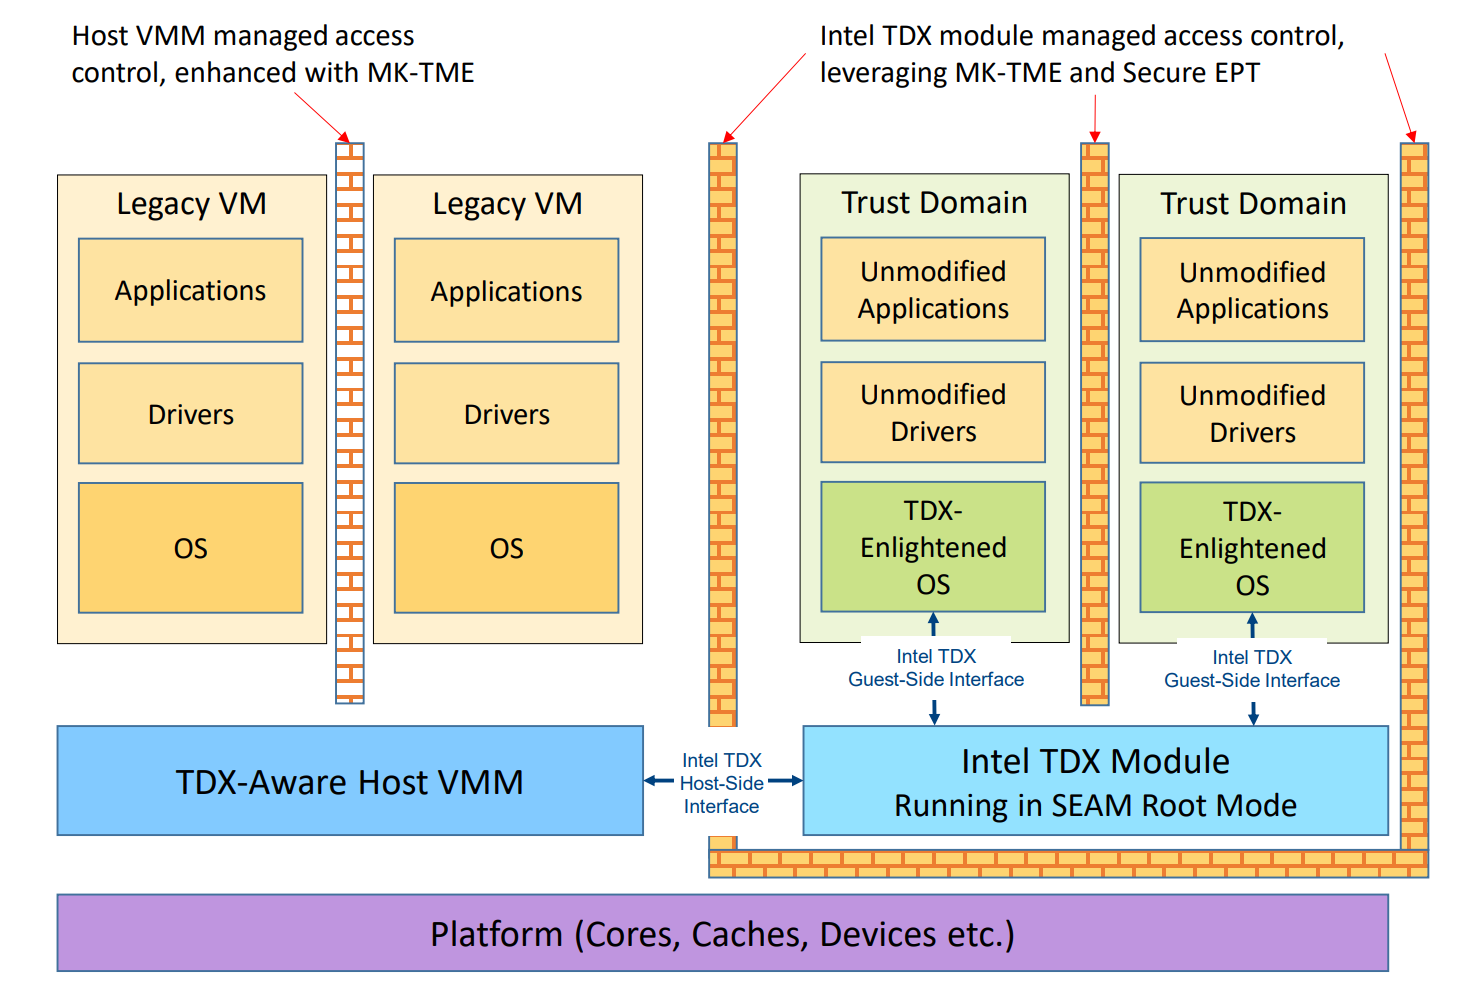
\includegraphics[width=\textwidth]{figures/TDX-Component-Overview}
\caption{TDX Component Overview taken from \cite[p.~19]{noauthor_tdx-module-10-public-specpdf_nodate}. Shown here is an extension of the Compute Stack in Fig. \ref{fig:computestack} with the colors corresponding to the non-TDX variants.}
\label{fig:component-overview}
\end{figure}
\begin{itemize}
    \item TDX-enabled processors, which offer combinations of the aforementioned capabilities.
    \item TDX Module, an Intel-signed and CPU-attested software module that leverages the features of TDX-enabled processors to facilitate the construction, execution, and termination of TDs while enforcing the security guarantees. These will be further looked at in the Threat Model in \cref{Threat_Model} and the Security Analaysis in \cref{Security Analysis}
\end{itemize}
Additonally it also shows the surrounding environment containing optionally normal VMs, the hardware and TDs ontop of the TDXM.The TDX Module provides two sets of interface functions, host-side interface functions for a TDX-enlightened hypervisor and guest-side interface functions for TDs. It is loaded and executed in the SEAM RANGE, which is a portion of system memory reserved via UEFI/BIOS. The P-SEAM Loader can install and update the TDX Module. More information on the loading process can be found in \cite{noauthor_white_nodate} and \cite{noauthor_tdx-module-10-public-specpdf_nodate}. The P-SEAMLDR will be discussed further in \ref{Security Analysis}.
The TDX-aware hypervisor operates in the conventional VMX root mode and uses the SEAMCALL instruction to invoke functions on the host side interface (function names start with TDH) of the TDX Module. Upon execution of the SEAMCALL instruction, the logical processor transitions from the VMX root mode to the SEAM VMX root mode and starts executing code within the TDX Module. Once the TDX module has finished its task, it returns to the hypervisor in VMX root mode by executing the SEAMRET instruction. On the other hand, TDs run in the SEAM VMX nonroot mode. TDs can trap into the TDX Module either through a TD exit by invoking the TDCALL instruction or triggered by some external event, e.g. an external interrupt or exception. In both cases, the logical processor transitions from the SEAM VMX nonroot mode into the SEAM VMX root mode and starts executing inside the TDX Module. \cref{fig:seamFigure} shows these transitions and their counter parts.

\begin{figure}
\centering
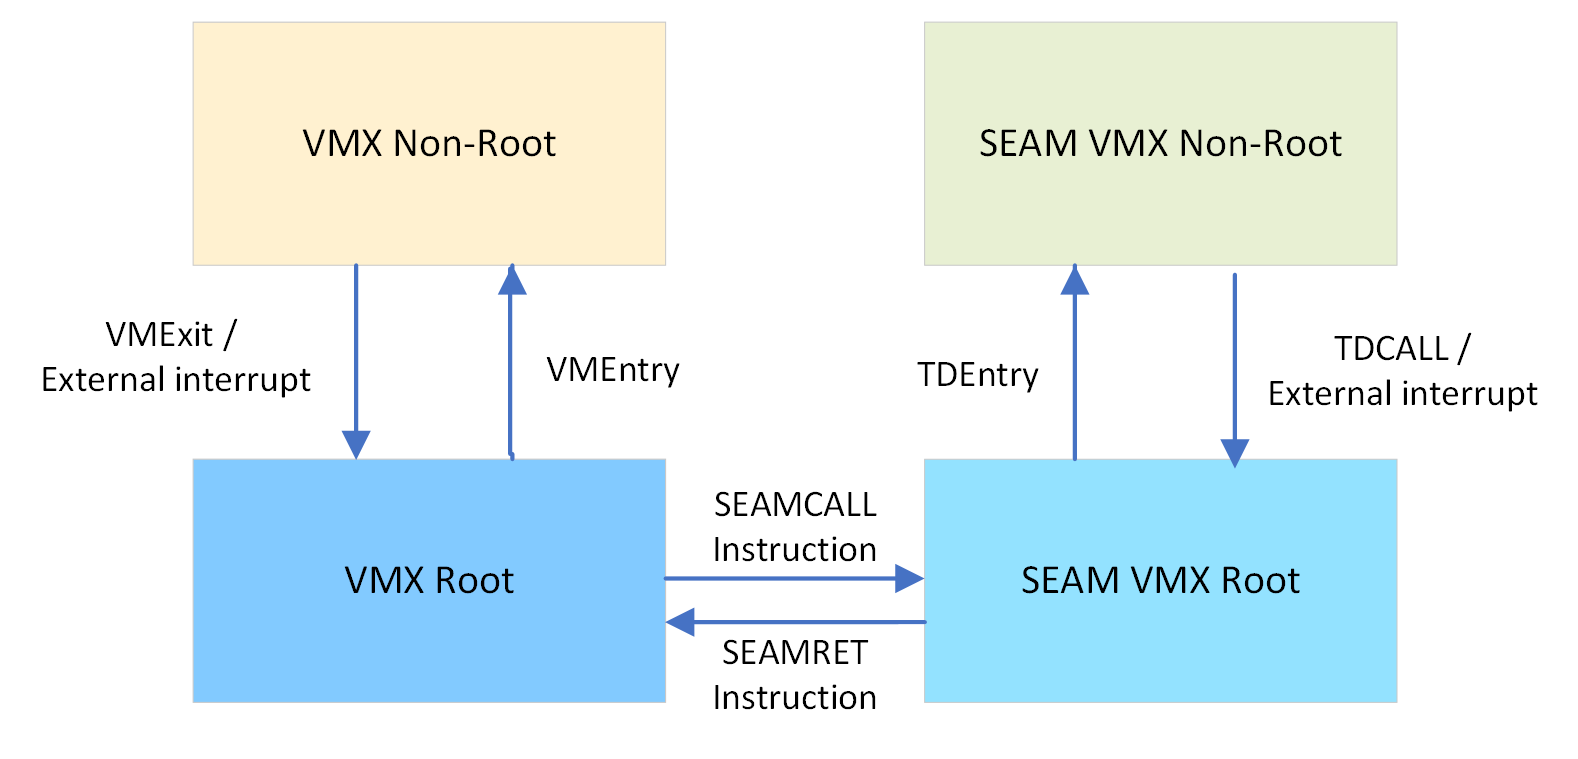
\includegraphics[width=0.7\textwidth]{figures/SEAMVMXÜBergänge.png}
\caption{VMX and SEAM VMX transitions. The colors are the same as they are for the implementations of these in \cref{fig:component-overview}. Note that it is not possible to transition from VMX non-root to SEAM non-root directly, as this would correspond to a direct transition from a TD to a non-TD vm.}
\label{fig:seamFigure}
\end{figure}
\subsection{TDX Key Generation and TD encryption}
The Host Hypervisor or Virtual Machine Manager (host VMM), which explicitly is not part of the TDX module but is aware of it calls the TDH.SYS.KEY.CONFIG function during startup, which configures the TDX modules global private key on the current CPU package \cite{intel_corporation_intel-tdx-module-15-abi-spec-348551001pdf_2024}. The host VMM can create a new guest TD by allocating and initializing a TD root control structure. The host assigns the TD a Host Key ID (HKID), which can be used to tag the memory accesses made by the TD\cite{noauthor_tdx-module-10-public-specpdf_nodate}. Subsequently, the host VMM calls the MKTME hardware, which encrypts the specified memory using a hardware-generated encryption key\cite{noauthor_multi-key-total-memory-encryption-spec-14pdf_nodate}. The VMM of the TD host configures the MKTME hardware by calling the TDH.MNG.KEY.CONFIG function on each CPU package. This will program the encryption key into the MKTME encryption engines\cite{noauthor_tdx-module-10-public-specpdf_nodate}. At this point, the TD private memory section is created and accessible by the TD. The VMM can then use Intel TDXM interface functions to create control structures. 

\subsection{The Threat Model}

\label{Threat_Model}

This section will outline the threat model, that is used in this thesis, as well as what Intel, in person of Andi Kleen and Elena Reshetova, outlined at \cite{elena_reshetova_intel_2023} sees as the TDX threat model.

\subsubsection{Adversarial Goals}

An attacker targeting TDX or a TD directly can focus on different components, depending on what their goals are. In general, they would be interested in leaking sensitive data or disrupting the expected behavior of a TD. These were also outlined by Aktas et Al. \cite{aktas_intel_nodate}.

\myparagraph{Leaking TD Secrets}

Once the TD has been verified via attestation, the owner of the TD usually provides confidential information to the TD. This could take the form of cryptographic keys, private user data, or similar. TDX aims to isolate this information from any malicious third party.

\myparagraph{Manipulating TD Behavior}

An adversary may be looking to change the behavior of a victim TD in various ways. As previously discussed the VMM can change some memory mappings the TD uses, which could lead to changes in the behavior of the application and faulty computational results.

\myparagraph{Host Denial-of-Service}

An adversary may aim to limit the availability of a cloud provider by obstructing the scheduling of other workloads (TDs, VMs) on a machine. This can be achieved by abusing the scheduler. Additional attacks can vary in their severity. For instance, a bug in a TD may lead to its shutdown, while a bug in the TDX module could necessitate an immediate halt of all TDs on the machine. Some memory states can cause unrecoverable machine checks which necessitates a full power cycle to recover \cite{aktas_intel_nodate}.

\subsubsection{Attack Vectors and Vulnerabilities}
In general attack categories, sometimes also called threat vectors, in scope for confidential computing according to the CCC are as follows:

\begin{itemize}
    \item \textbf{Software Attacks} aimed at firmware and software on the host and also software inside the TEE
    \item \textbf{Protocol Attacks} on the attestation protocols and data in transport
    \item \textbf{Cryptogrphic Attacks} against ciphers and algorithms, for example hashing or encryption algorithms
    \item \textbf{Basic physical attacks} such as \guillemotright cold DRAM extraction, bus and cache monitoring and plugging of attack devices into an existing port \guillemotleft \cite{confidential_computing_consortium_ccc--technical-analysis--confidential-computing-v13_unlockedpdf_2023}
\end{itemize}

The threat model does not address any threats made possible by the TDX guest userspace directly using TDVMCALL hypercalls (through the TDX-module) and shared memory for IO exposed to an untrusted host/VMM. If TDX guest userspace enables debug or test tools that can read memory-mapped I/O (MMIO) or PCI configuration space without validating the input from untrusted host/VMM, it opens up the possibility of many more attacks. In addition malicious input from, for example,  PortIO, SharedMemory or KVM Hypercalls is consumed from the host by device drivers in the TD, which are implicitly trusted and part of the TCB. If those drivers are vulnerable this can lead to threats from inside the TD, although Intel has provided mitigation measures against those \cite{elena_reshetova_intel_2023}.

According to Intel the TCB contains only a few components:

\begin{itemize}
    \item Intel TDX module, with Persistent Seam Loader (P-SEAMLDR) an Non-Persistent Seam Loader (NP-SEAMLDR)
    \item Intel Authenticated Code Modules (ACM), for example the BIOS ACM
    \item TD Quoting Enclave
    \item Intel CPU Hardware
\end{itemize}

All other components, such as the BIOS, SMM, host OS, and the VMM, are situated outside the TCB \cite{noauthor_tdx-whitepaper-february2022pdf_nodate}.


The TCB for Intel TDX has a restricted number of system components, which creates only a few opportunities for adversaries to breach system security. Moreover, when a malicious Virtual Machine Manager (VMM) and a malicious TD work together, they can exploit complex scenarios that the system designers may not have foreseen. The following will give a quick summary of the attack vectors from \cite{aktas_intel_nodate} and then describe two additional vectors, which are more prevalent for the issues at hand.

\myparagraph{Intel signed Software}

Even though the TCB is small, Intel has to build a chain of trust from its own hardware and the BIOS to the TDX Module and the guest TDs. It does that by using different open and closed source layers of signed code the system has to go through before it is fully booted. With the BIOS being outside the TCB, TDX has to make sure that all security-sensitive settings are within an acceptable range. Intel has developed MCHECK for this. MCHECK is situated inside the CPU microcode and is not made public by Intel, it is thus completely opaque to the user. Next, during the Host startup NP-SEAMLDR and P-SEAMLDR are loaded by trapping into the SEAM root-mode mentioned in \cref{TDX Architecture}. NP-SEAMLDR prevents the BIOS from executing any further. NP-SEAMLDR then loads P-SEAMLDR which in turn loads the TDX Module, which is the central privileged software component for runnings TDs. The security of these has been looked at and verified by Aktas et Al. prior to TDX beining released \cite{aktas_intel_nodate}. They have discovered at least ten different, software-based, security issues, which have been fixed now. One of these attacks allowed arbitrary code execution inside elevated SEAM root-mode, which would completely cancel any security guarantees by Intel. A malicious TD can only attack via the TDX Module, which if compromised would grant complete access to the TD. As of the writing of this thesis Intel has not published any security advisories regarding TDX \cite{security_advisories}.

\myparagraph{Hardware attacks}

Intel considers \guillemotright opening the case and tampering of [sic!] internal hardware to compromise SGX is out of scope for SGX threat model. \guillemotleft \cite{chen_voltpillager_nodate}. As outlined in \cref{sec:tdxBuildingBlocks} TDX relies on SGX for its security, thus vulnerabilities in SGX can also affect TDX. The threat model for Confidential Computing contains basic hardware attacks, with the difference between basic and complex hardware attacks being unclear. The amount of preparation and additional hardware needed appear to be a differentiating factor, some basic hardware attacks can be prevented via software precautions but both are only completely prevented by preventing direct hardware access. 

\myparagraph{Outside connection to the TD}

The last major interface is the outside connection to the TD. Here two different problems arise. Making sure that data is not compromised in transit is technically not part of the threats TDX wants to protect against and it does not itself do so,  but it can help with establishing a secure connection. The second issue that comes up is making sure that communication is done with the correct TD. TD identity checking is explicitly outside the scope of TDX but it can help with that and this will be another concern in this thesis. The TDX attestation only guarantees that somewhere a TD runs on certified hardware with a signed TDX Module version. Additional information the Quote can supply will be needed to identify a TD. Without a secure connection a TD remains useless, as any results it calculates, can not be consumed by an outsider. An exemplary man-in-the-middle attack is shown in \ref{fig:man_in_the_middle}.
\begin{figure}
   \centering
       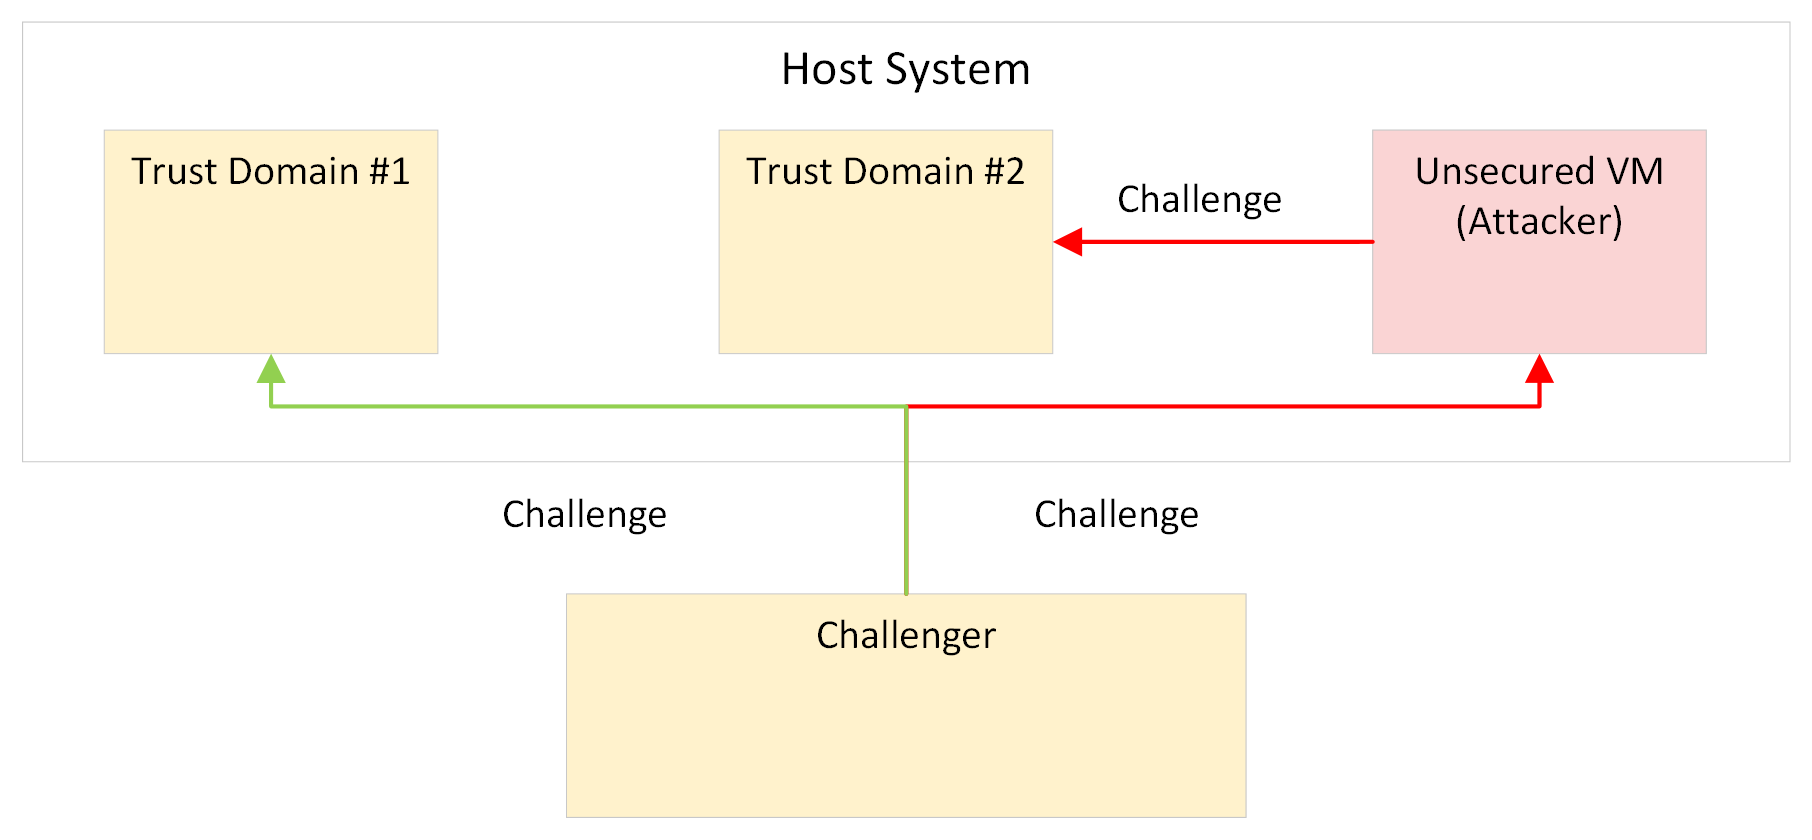
\includegraphics[width=.75\textwidth]{figures/Man-In-The-Middle.png} 
 \caption{A simple man-in-the-middle attack against a TD. The attacker reroutes the challenge to an unsecured VM, which in turn requests a quote from a different TD}
 \label{fig:man_in_the_middle}
\end{figure}
Provided that security promises within the previously mentioned parts of the TCB are solid, connecting to and verifying the identity of a \Gls{TD} is the last step towards secure computation with user Input.

\subsubsection{Threats TDX does not protect against}

Some threats and attacks that are explicitly outside the threat model of TDX. For some of these TDX might hinder the effectiveness or even prevent them but it does not try do that.

\myparagraph{Side-Channel Attacks}

Side-Channel Attacks are attacks that take advantage of unintended output channels of a system. The first documented one was when in 1965 MI5 tried to decipher a cryptography device used in the Egyptian Embassy \cite{zhou_side-channel_nodate}. To reduce the computational effort, they listened to the setting of the device through a microphone placed close to a window, and thus deduced the position of some of the machine's rotors.
By their nature TDX can not protect against all Side-Channel attacks, but importantly, it is effective against all currently known forms of the "Spectre-Family" attacks. Explicitly outside the scope of the TDX threat model are computation-time and power-analysis attacks, as well as studies from memory access patterns.

\myparagraph{Vulnerable Applications}

The guest Operating System is part of the \Gls{TCB} but is not under the control of the TDX creators or developers. Any issue within an \Gls{OS} can cause issues within a \Gls{TD}. This would also happen with a server that is hosted on your own premises and not  and is thus not being protected against. Similarly, any security issue within an outward facing application within a \Gls{TD} is a security issue that can not be fixed by using TDX. This means that an application inside a TD is at most as secure as the application itself. 


\subsection{TDX Attestation}
\label{TDX attestation}
Hardware attestation is a process that establishes the integrity and trustworthiness of hardware components in a computing system. It involves verifying the identity and expected behavior of hardware components connected to the motherboard. It can be used standalone, but also in connection with software attestation. Software attestation can measure parts, or the entirety, of the memory and report these measurements to a remote party, which can then verify those measurements \cite{stumpf}. This verification is done by checking identification codes and comparing them to expected values. Software attestation can use hardware attestation as an anchor for its chain of trust. Attestation is necessary to establish trust for a challenger that the used hardware is as expected. Hardware and software attestation can be used to establish trust into a remote platform for a challenger.
The TD attestation protocol involves six key entities: the Quoting Enclave (QE), the host Virtual Machine Manager (VMM), the guest trust domain (TD), the Intel TDX module, the CPU hardware and the challenger. The QE is an Intel-provided enclave that signs the report body after its successful verification to create a remotely verifiable quote. The VMM is an untrusted hypervisor that manages Virtual Machines. The guest TD is an enhanced Virtual Machine that is initialized and measured at boot time. The TDX module is Intel-provided software that is signed by Intel and manages the interaction between the TD and the VMM. It is also part of the attestation metadata. The CPU hardware generates and verifies the report. Lastly, the challenger (also known as the relying party) is the remote party that performs the attestation verification.


\label{Pre-Attestation setup}
Before any attestation challenge request can be answered the platform itself must be registered at the Intel Provisioning Certification Service \cite{intel_corporation_dcap_2024-1}. This is done by creating an asymmetric shared platform key using the hardware-keys of the different CPUs on the platform. It is shared between the different CPUs. This shared platform key is then encrypted using those hardware-keys and safed on the NVRAM of the BIOS. After booting the host platform accesses a platform certificate via the Provisioning Certification Enclave (PCE), which is signed using the shared key created previously. The host then has to register the platform at the Provisioning Certification Service (PCS). During this registration Intel checks the validity of the platform manifest. If verified the PCS returns a certificate for the platform key to the PCE \cite{cheng_intel_2023}. The result can be cached locally using an implementation of the Intel provisioning certification caching service \cite{caching_service}. Next the Trusted Domain Quoting Enclave (TD QE) needs to have its own key signed. The TD QE is an an SGX-enclave running on the Host, which later signs the TD quotes during the TDX attestation. The PCE now needs to establish that the TD QE is running on the same platform as it is, this is done via local attestation. Secure connection between two SGX enclaves is explained in more depth in \cite{intel_corporation_migration_spec_2023}. The local attestation is shown in \cref{fig:local-attestation}. The steps needed are as follows:
\newcommand\setItemnumber[1]{\setcounter{enumi}{\numexpr#1-1\relax}}
\begin{enumerate}
    \item The TD QE generations an asymmetric key-pair called attestation key (AK)
    \item The TD QE sends a request for local evidence to the CPU hardware. This request includes the hash of the public part of the previously generated AK combined with any additional user provided authentication data. Intel does not provide information if this is filled. Additionally the TD QE has to specify the verifying enclave as the PCE.
    \item The CPU packs this information and claims about the TD QE and MACs it using the Report Key (RK) into the QEReport.
    \item The QEReport is returned to the TD QE
    \item The TD QE forwards the QEReport and its public AK to the PCE
    \item[6. \& 7.] The PCE requests the RK from the CPU hardware
\setItemnumber{8}
    \item The PCE verifies the evidence based on the policy set by the PCE owner. This includes at least verification of the MAC over the QE Report Body and the hash of the public AK.
    \item The PCE then signs the claims using the PC Key and returns this to the TD QE. According to \cite{scarlata_supporting_nodate} the so-called AK cert is a cert-like structure identifying the QE and the Attestation Key, they do not further specify how the certificate is made up but according to \cite{sardar_formal_spec_ARM_2024} it contains the public AK, the QEReportBody and the signature PCKsig over the QEReportBody.
    
\end{enumerate}

\begin{figure}
\centering
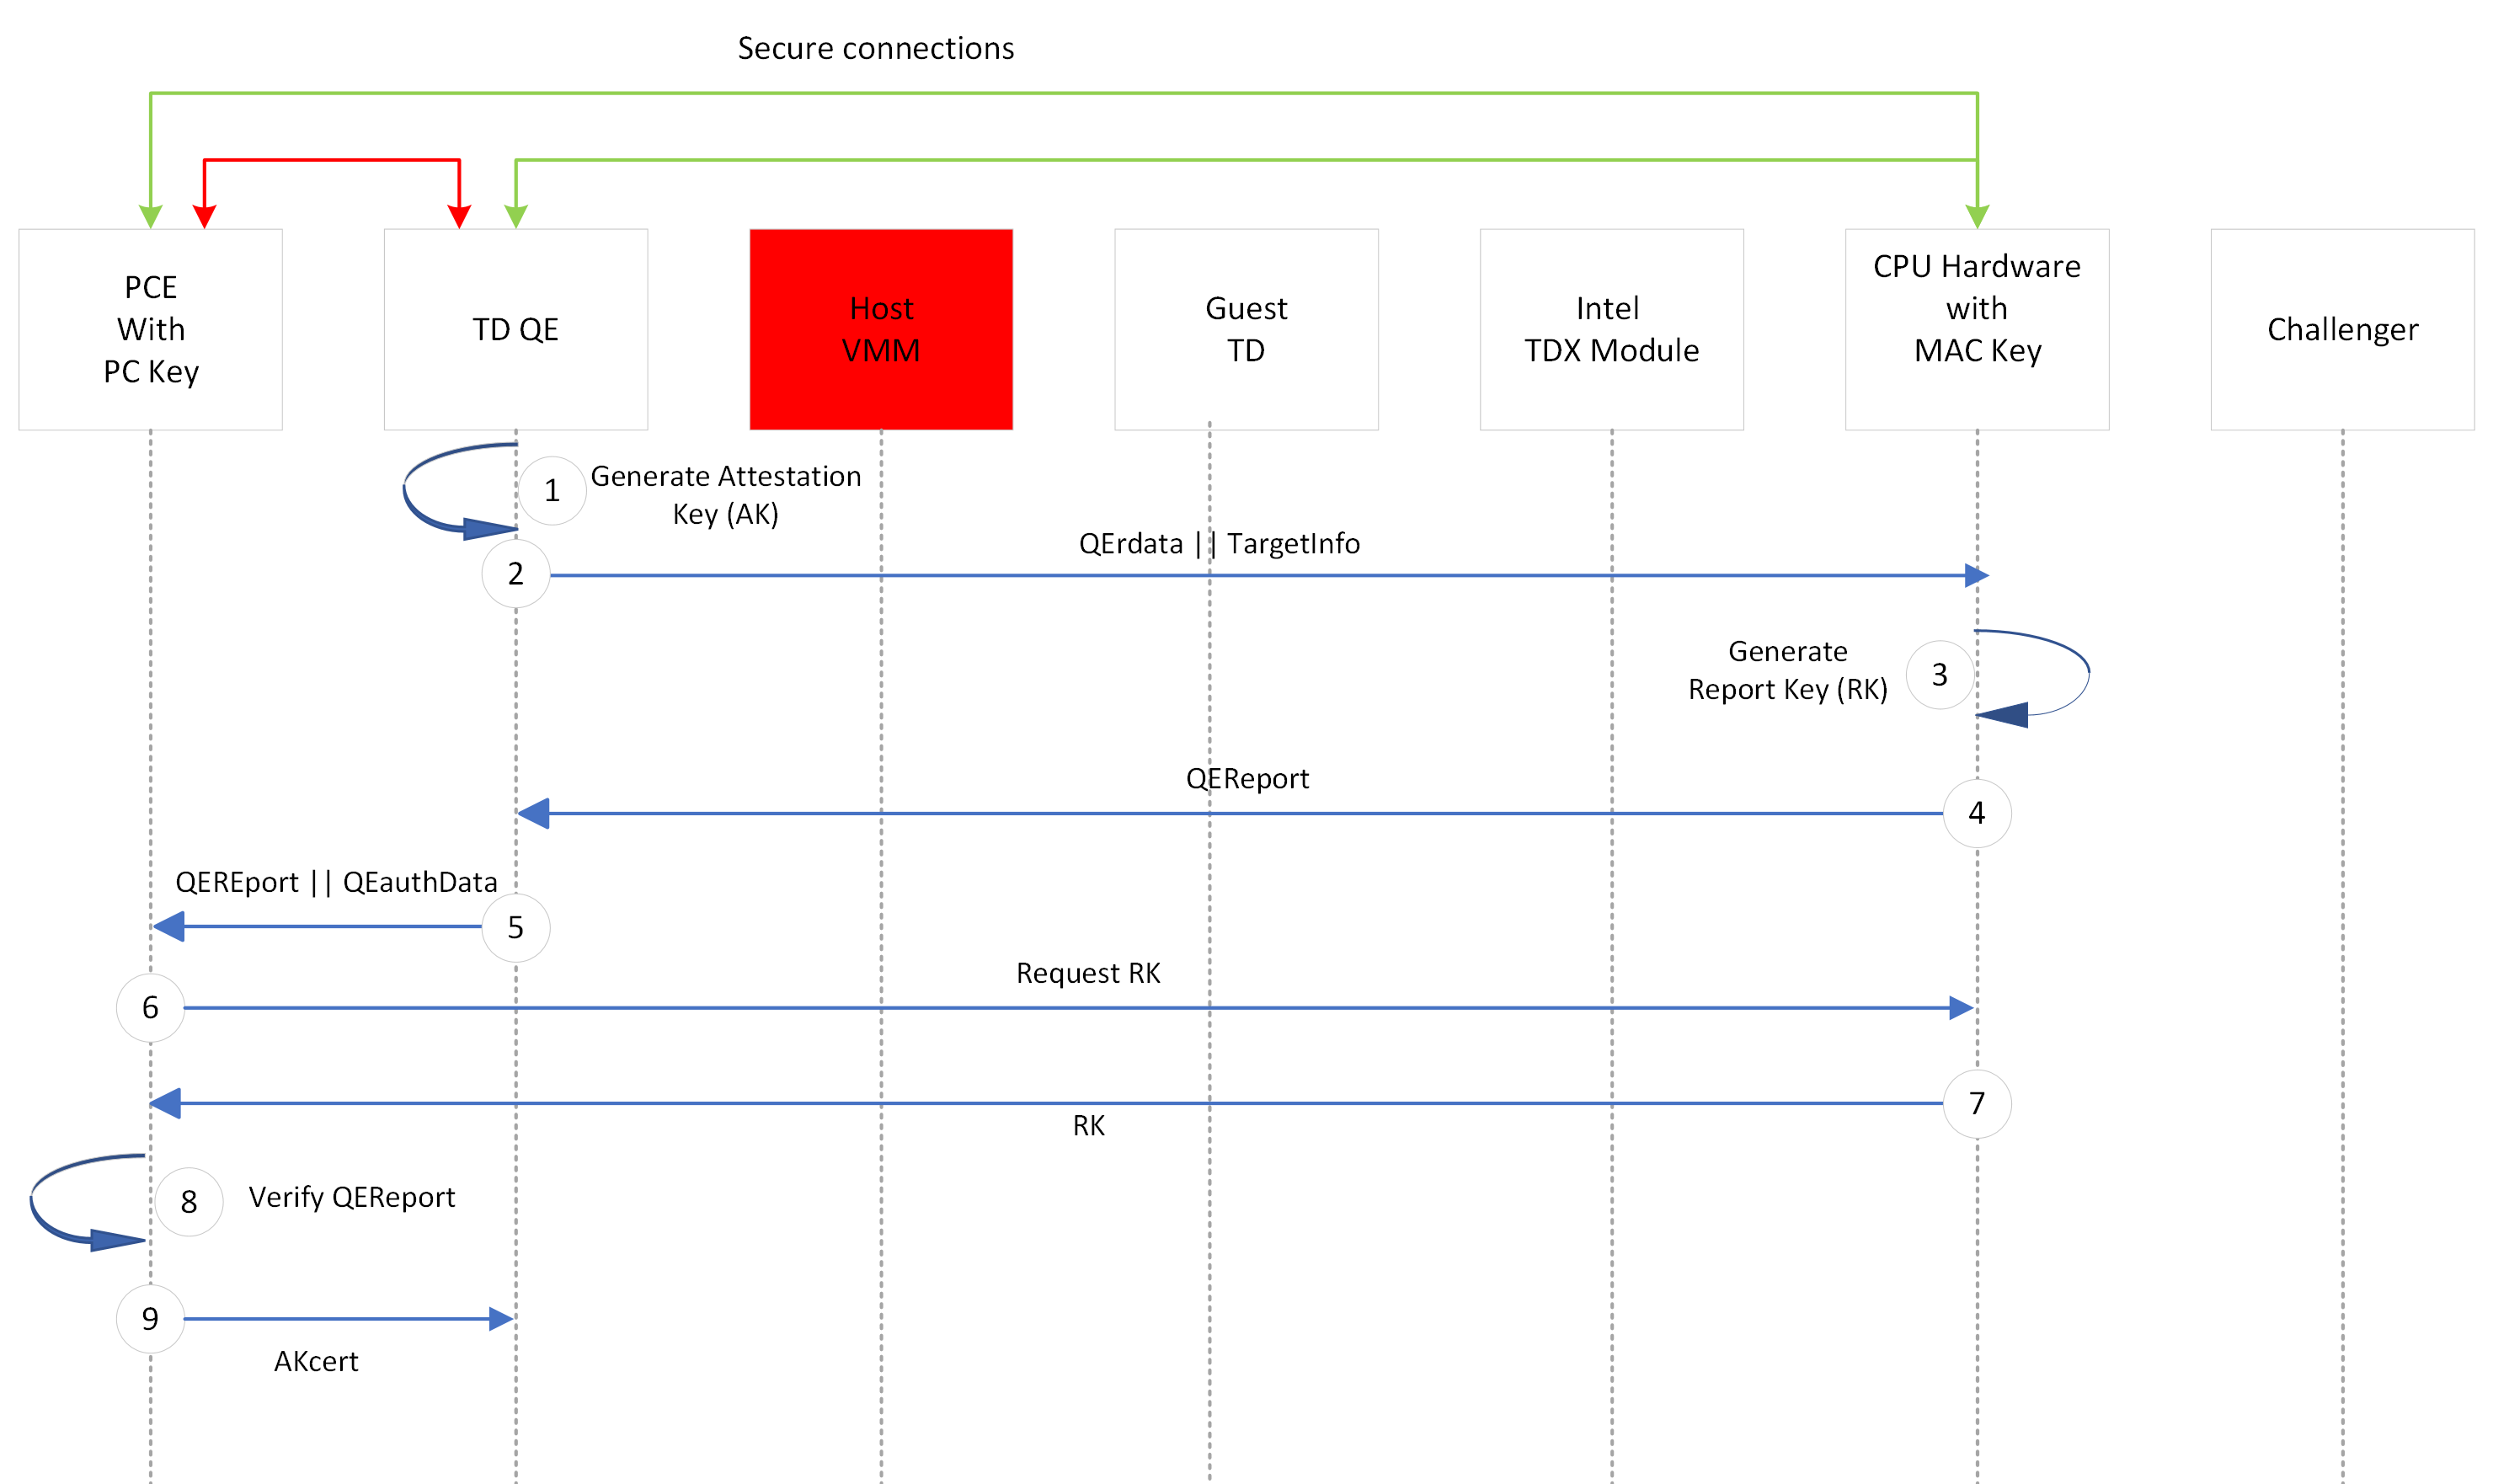
\includegraphics[width=0.9\textwidth]{figures/Local Attestation.png}
\caption{Intel TDX local attestation flow diagram. Text above the arrow represents data being sent, text below function calls. The Host VMM in red is untrusted. The challenger is shown to have the same entities as \cref{fig:QuoteGeneration}. Adapted from \cite{sardar_formal_2023}}
\label{fig:local-attestation}
\end{figure}

Complementary to the three requirements required by the Confidential Computing Consortium, in attestation generally according to \cite{sardar_demystifying_2021}, adapted to fit with TDX attestation vocabulary, the four most interesting properties are:

\label{FourProperties}
\textit{Integrity}: Claims within the TD quote, represent the present condition of the TD and contain verifiable components such as identity fields. Therefore, it is crucial to prevent an adversary from altering claims while they are being transported from the TD to the challenger. Typically, the integrity of claims is safeguarded through digital signatures utilizing an Attestation Key. If integrity holds, then it means that the adversary cannot modify claims inside the TD quote without being detected.

\textit{Freshness}: Freshness means that the TD Quote is the latest created quote to a specific request. The freshness of Evidence is crucial because otherwise an attacker potentially has the ability to replay authentic Evidence from a previous session while also altering the state of the TD.


\textit{Authentication}: The challenger must ensure it communicates with the intended TD. Informally, if the Verifier receives the public key of the TD, this uniquely matches the public key generated within the TD. This implies that the adversary does not have access to keys or secrets related to the attestation shared between the TD and the challenger, which is called secrecy.

Hardware attestation establishes trust in the hardware, but not in the software being executed. The Attestation does however generate a quote that contains additional information on the TD and the software being executed. Trusting the Quote does not mean trust with the TD is established. This establishes the environment of the TD, mainly the specific hardware and the TDX Module. With the additional information about the VM and the Image in the Quote verification might be possible but the implementation of that is left to the software developer. More information on this can be found in \cref{Identity}.
\begin{figure}
\centering
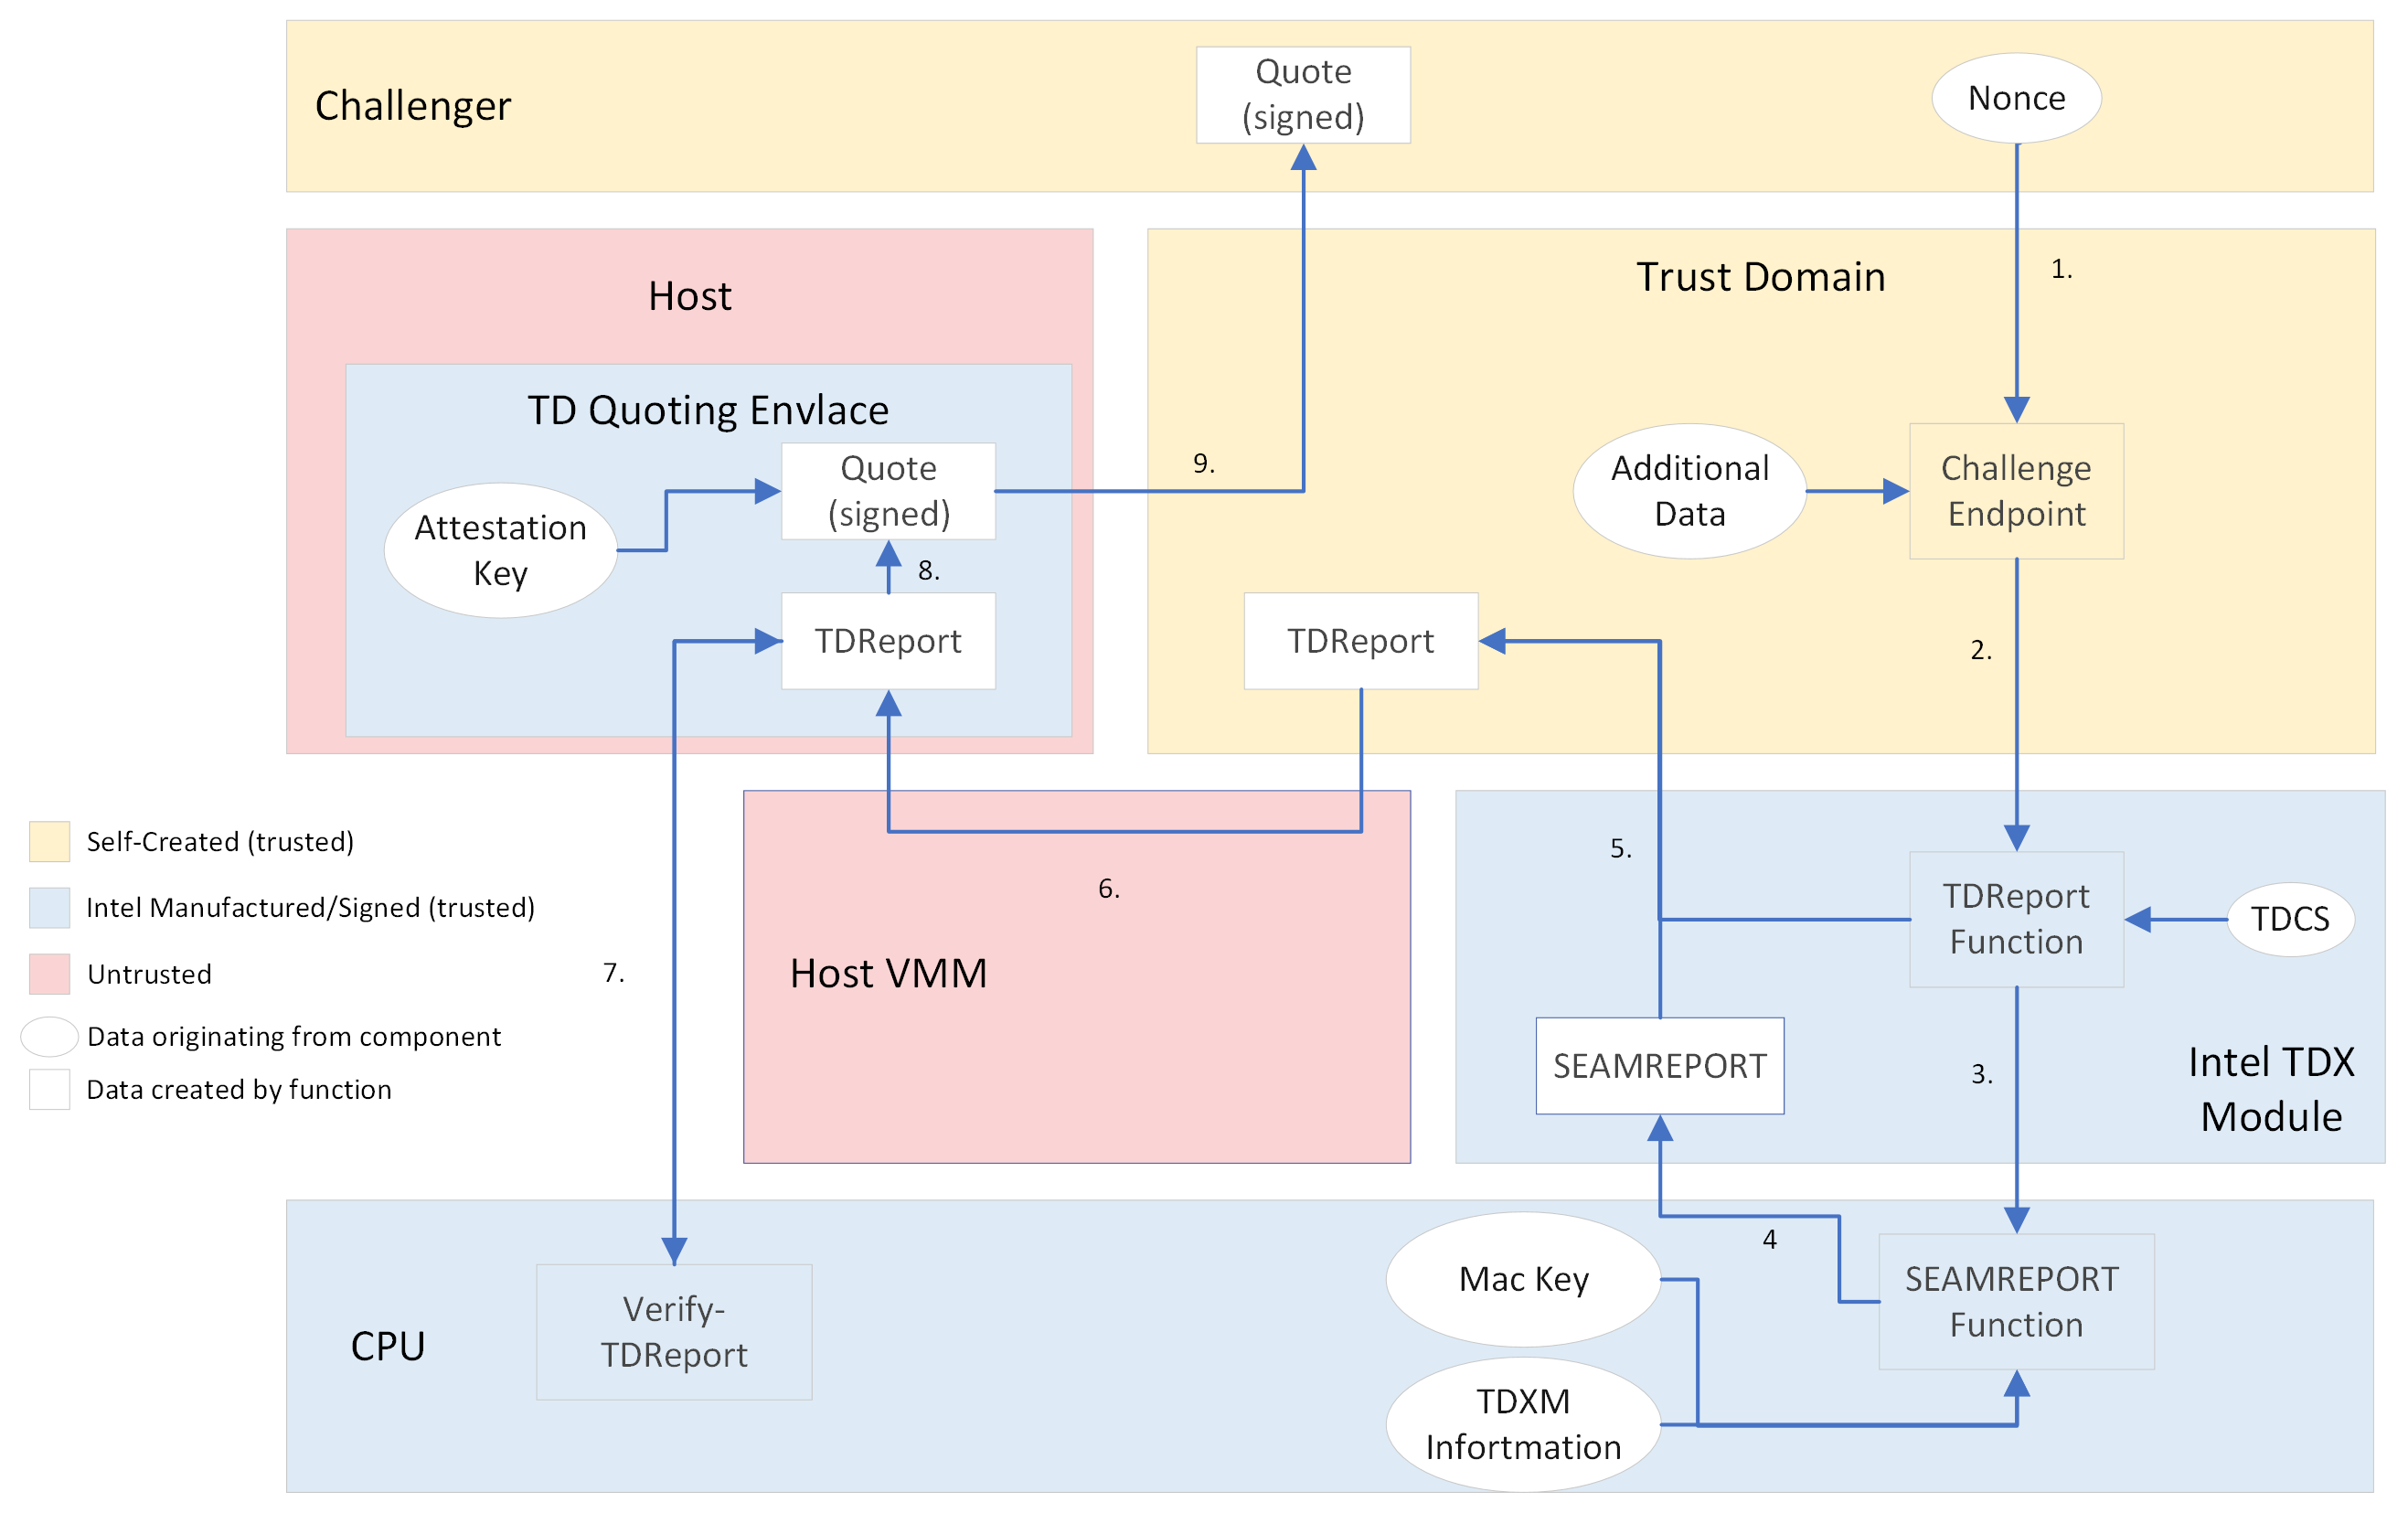
\includegraphics[width=\textwidth]{figures/Attestation-einfach.png}
\caption{A simplified SGX-based TD attestation flow. Adapted from \cite[p.~111]{noauthor_tdx-module-10-public-specpdf_nodate}}
\label{fig:EasyAttestation}
\end{figure}
Figure \ref{fig:EasyAttestation} shows a rudimentary TDX attestation flow with trusted and untrusted entities as well as their boundaries. The challenger requests a quote from the guest TD for challenge. He can include a one-time key, called nonce to prevent replay attacks. A quote is all the information necessary to attest to a specific set of hardware. After receiving the request the guest TD can supply additional runtime data, which is important to verify the identity of the TD, and will then send a request via a character device to the TDX module. This report contains data the TDX module holds about the TD, most importantly measurements relating to the creation of the TD, and the data that was supplied by the TD. To prevent a data breach during the data transfer via the untrusted Host VMM the CPU has a Message Authentication Key (MAC) from the TD QE, which it uses to MAC the TDReport. The TD QE now calls the CPU again to verify the integrity of the TDReport.
To create a chain of trust, which can only be accessed via Intel, the Attestation key was previously signed by the PCE key, which was signed by Intel. 

\begin{figure}
\centering
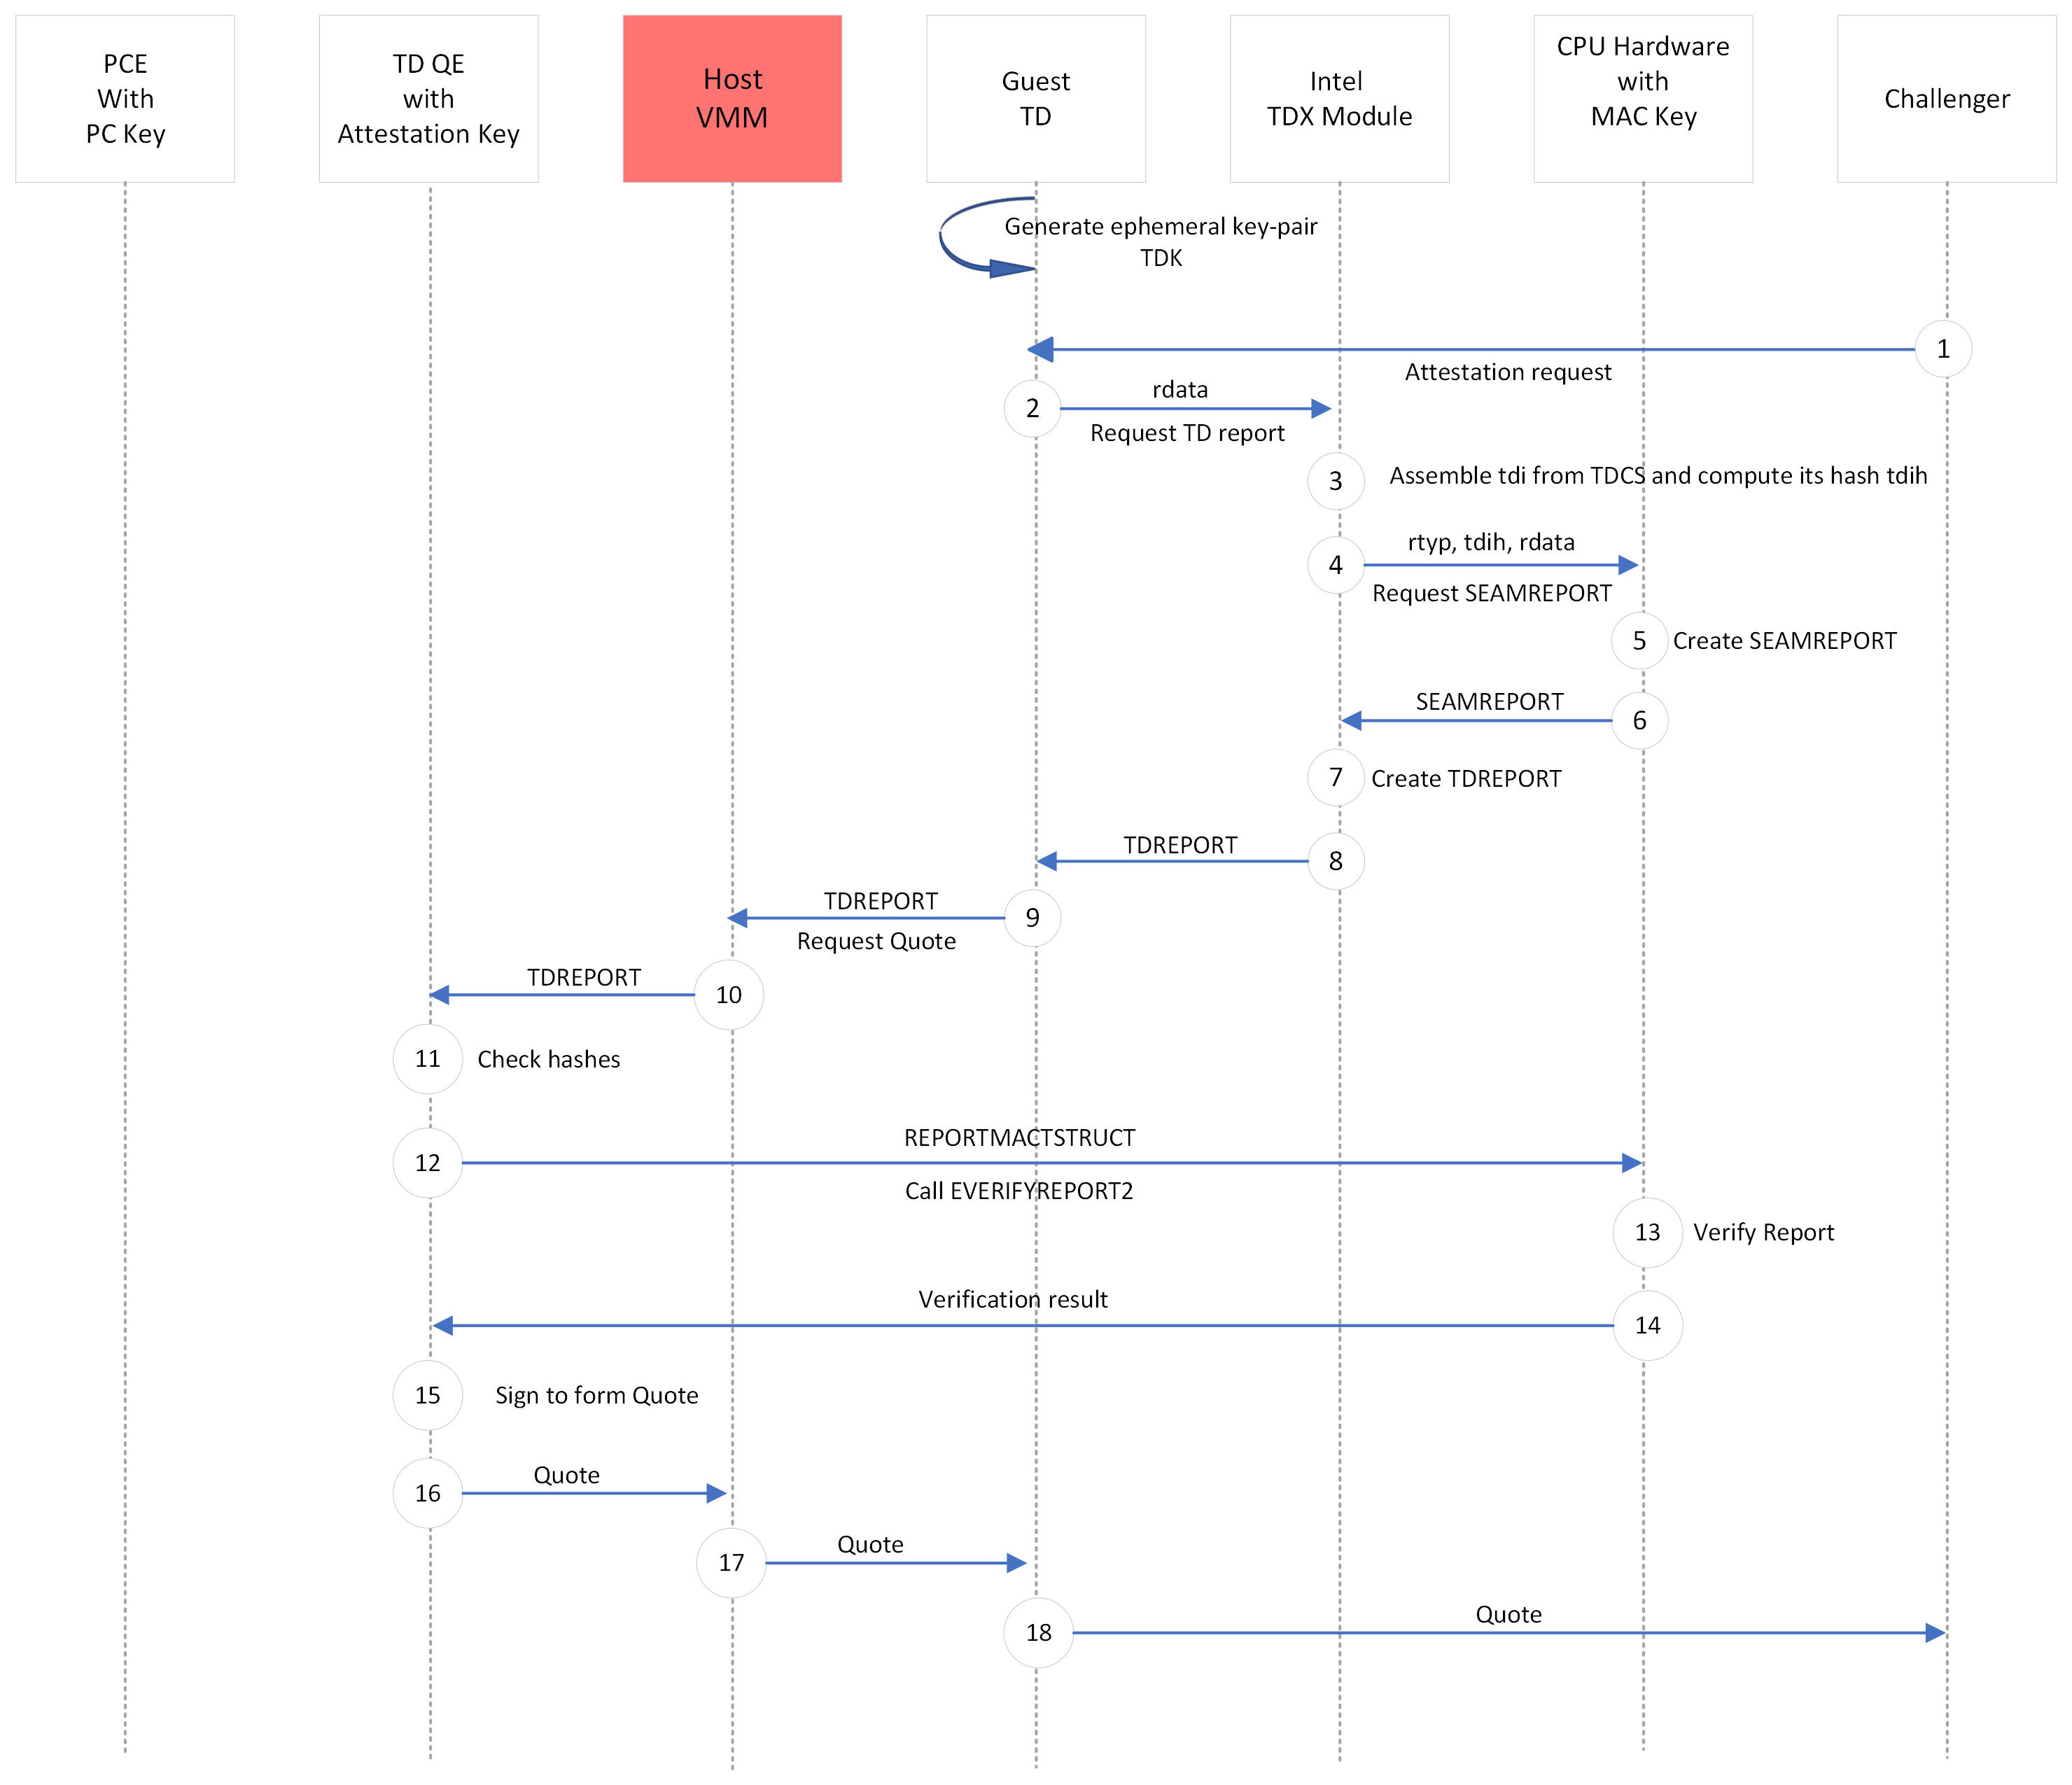
\includegraphics[width=\textwidth]{figures/Attestation Diagram.png}
\caption{Intel TDX Attestation flow diagram. Text above the arrow represents data being sent, text below function calls. The Host VMM in red is untrusted. The PCE is shown to have the same layout as \cref{fig:local-attestation}. Adapted from \cite{sardar_demystifying_2021}}.
\label{fig:QuoteGeneration}
\end{figure}
The following will now explain each step in more technical detail, while using Figure \ref{fig:QuoteGeneration} as reference. 
TDX includes a set of major functions explained here. \textit{Sign} represents the Elliptic Curve Digital Signature Algorithm signature over the message with the specified signature key. 
Calculating the \textit{hash} means computing the SHA384 hash of the input. \textit{Hmac} is HMAC\_SHA256 of the message with the specified key. More information on hmac can be found in \cite{hmac_keying_1996}. The message is not extractable if hmac is considered a pseudorandom function, which in practice appears to be true\cite{bellare_new_2006}. The TDK key-pair is sometimes also called TD key-pair.
\begin{enumerate}
\item The challenger initiates the attestation process by sending a challenge request to the Guest TD. This can include a nonce to prevent replay attacks\cite{sardar_formal_2023}.
\item The TD calls the TDG.MR.REPORT function to initiate the attestation on the system. It can specify any additional data in the REPORTDATA field, called rdata from here. On Linux this can be done via the character device tdx\_guest. This triggers a TDExit as shown in \cref{fig:seamFigure}
\item TDXM assembles TD information data structure tdi from Trust Domain Control Structure (TCDS) and computes its SHA384 hash tdih. The TCDS contains the following information:
\begin{itemize}
    \item Fields designed to control the TD operation as a whole (e.g., a counter of the number of VCPUs currently running). 
    \item Fields designed to control the execution control of the TD (debugability, CPU features available to the TD, etc.). 
    \item Registers filled with static and runtime measurements. 
    \item EPTP: as designed, a pointer (HPA) to the TD’s secure Extended Page Table (EPT) root page and EPT attributes
    \item Model Specific Register (MSR) bitmaps, designed to be used by all the TD’s VCPUs. 
    \item A page filled with zeros, designed to be used in cases where the Intel TDX Module needs a read-only constant 0 page encrypted with the TD’s private key.
\end{itemize}
\item TDXM calls the SEAM instruction SEAMREPORT with tdih and rdata
\item[5. \& 6.] CPU generates the SEAMREPORT, smr with a MAC block of hashes and the report data called rms and the TDX module measurements called tcbi. They are respectively red and purple in \cref{fig:tdr}. It then returns that report to the TDX module. This importantly contains measurements about the TDX module and about the TDX module signer, in this case Intel.
\setItemnumber{7}
\item TDXM builds the TDRreport tdr with the smr, a reserved block of memory, and the tdi created in step 3. Content for the entire tdr can be seen in Figure \ref{fig:tdr}
\begin{figure}
\centering
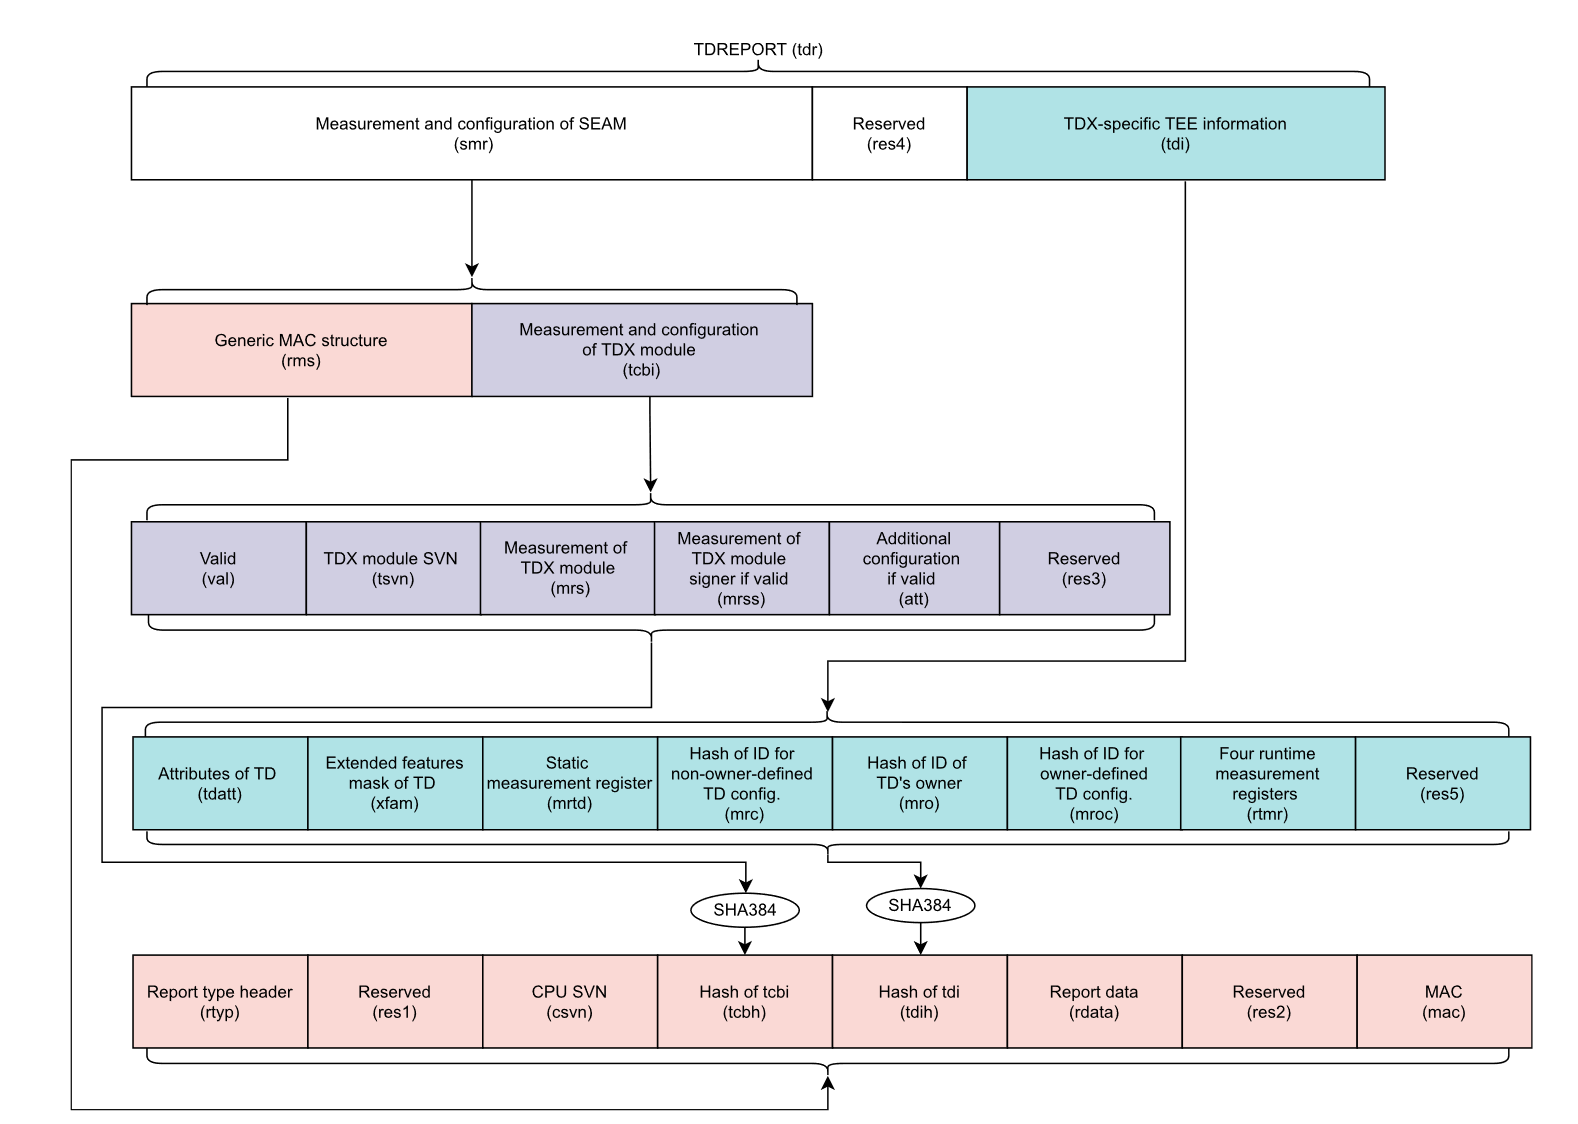
\includegraphics[width=\textwidth]{figures/tdr.png}
\caption{An overview of the component of the TDREPORT taken from \cite{sardar_demystifying_2021}}
\label{fig:tdr}
\end{figure}
\item TDXM sends tdr to the Guest TD
\item[9 \& 10.]The Guest TD sends tdr to the TD Quoting enclave, via the untrusted VMM
\setItemnumber{11}
\item TD QE verifies the hashes in report
\item Rms (part of smr, red in Fig \ref{fig:tdr}) is used as an argument in the 
ENCLU[EVERIFYREPORT2] cpu function. 
\item[13. \& 14.] CPU performs the verification of rms and returns the result to the TD QE. The verification consists of three main steps: 
\begin{enumerate}
\item verify that the header rtyp in the report is correct, 
\item verify that the CPUSVN is a valid value, and 
\item compute the MAC over the fields in the report body rptbody using the MAC key MACkey, and verify that the computed MAC matches the value in the field mac of the received report (represented as receivedMAC)
\end{enumerate}
\setItemnumber{15}
\item TD QE replaces the MAC in the rms with <rptbody, (sign(AK, rptbody))> to create a complete quote.
\item[16. \& 17.] Quote is sent to TD, VMM is untrusted → Sent by public channel
\setItemnumber{18}
\item TD sends quote to relying party(RP)
\end{enumerate}
The challenger can now verify the Signature on the Quotebody by going back the chain of trust rooted at Intel. This verification is based on the Data Center Attestation Primitives (DCAP) which will be explored later on in \ref{Security Analysis}. After verification the challenger can now send a secret encrypted with the public key of the TD to the TD establishing a common secret for further secure communication. If the TD did not include a public key in its quote section \cref{Establishing_a_secure_connection} contains further information on how to establish a secure connection. According to \cite{sardar_formal_2023} using ProVerif, this ensures integrity for the tcbi, tdi and rdata. It also ensures freshness and secrecy. Authentication does old as long as secure communication via TLS or similar is not established, which will be looked at in \cref{Establishing_a_secure_connection}.Ihc gu

\section{Related Work}
TDX has been looked at a fair amount of times already. In particular, a nearly complete security analysis of its hardware and the low-level TDX software by Aktas et al. at Google \cite{aktas_intel_nodate}. They limited their analysis to just the host-side without looking at TD user or developer issues down the line. Similarly, Sardar et al. formally verified TDX attestation in \cite{sardar_demystifying_2021}. They looked at the theoretical security of a perfect implementation. Knauth et al. introduced a way to create a secure channel using Intel SGX \cite{knauth_integrating_2019}, this will be used as the basis to establishing a secure channel to the TD in this thesis. Cheng et al. briefly mention this as well, but their focus was more generally on the TDX architecture \cite{cheng_intel_2023}. This thesis explores the feasibility of those for an average user, as well as its security assumptions and pitfalls. Lefeuvre et al. have looked at difficulties and issues with safe and confidential I/O \cite{lefeuvre_towards_2023}, this will only be briefly touched upon in this thesis. Delignat-Lavaud et al. looked at issues pertaining the TCB of confidential services. Their information was used in this thesis to look at the feasibility of using CC for the average user. Their consensus was picked up in this thesis that while CC is great in theory, the practice is lacking.

